% graph theory and combinatorics — a short LaTeX lesson
%
% This is a real, compilable .tex file, not a markdown note — pt's LaTeX
% support works on any .tex file directly. Right-click this file in the
% sidebar and choose "compile LaTeX -> PDF"; it runs the system's pdflatex
% twice (so the numbered theorem/example cross-references settle) and opens
% the resulting PDF in the built-in viewer. You need a TeX distribution
% installed (TeX Live, MacTeX, or MiKTeX) with pdflatex on PATH — if the
% compile fails with "could not run pdflatex", that's the thing to install.
%
% If your TeX install doesn't include TikZ, delete the \usepackage{tikz}
% line and the tikzpicture block in section 3 — everything else compiles
% without it.

\documentclass[11pt]{article}
\usepackage[margin=1in]{geometry}
\usepackage{amsmath, amssymb, amsthm}
\usepackage{tikz}

\newtheorem{theorem}{Theorem}[section]
\newtheorem{lemma}[theorem]{Lemma}
\newtheorem{corollary}[theorem]{Corollary}
\theoremstyle{definition}
\newtheorem{definition}[theorem]{Definition}
\newtheorem{example}[theorem]{Example}

\title{Graph Theory and Combinatorics: A Short Course}
\author{lessons/07-latex-graph-theory.tex}
\date{}

\begin{document}
\maketitle

\section{Graphs, formally}

\begin{definition}
A \emph{graph} $G = (V, E)$ consists of a set $V$ of \emph{vertices} and a
set $E$ of \emph{edges}, each edge being an unordered pair of vertices. The
\emph{degree} of a vertex $v$, written $\deg(v)$, is the number of edges
incident to it.
\end{definition}

This is deliberately the same abstraction Euler used in 1736 to solve the
Seven Bridges of K\"onigsberg problem — see \texttt{04-academic-book.md} for
the historical version of this same story, told in prose with footnotes
rather than theorems.

\section{The handshake lemma}

\begin{theorem}[Handshake lemma]
For any graph $G = (V, E)$,
\[
  \sum_{v \in V} \deg(v) = 2|E|.
\]
\end{theorem}

\begin{proof}
Each edge $\{u, v\} \in E$ contributes exactly $1$ to $\deg(u)$ and exactly
$1$ to $\deg(v)$ — so it contributes exactly $2$ to the sum
$\sum_{v} \deg(v)$ in total. Summing over all $|E|$ edges gives $2|E|$.
\end{proof}

\begin{corollary}
Every graph has an even number of vertices of odd degree.
\end{corollary}

This corollary is exactly why no walk crossing every K\"onigsberg bridge
exactly once could exist: all four landmasses had odd degree, and a walk
using every edge once needs at most two odd-degree vertices (its endpoints).

\section{Euler's formula for planar graphs}

\begin{theorem}[Euler's formula]
For a connected planar graph drawn without crossing edges, with $V$
vertices, $E$ edges, and $F$ faces (including the unbounded outer face),
\[
  V - E + F = 2.
\]
\end{theorem}

\begin{example}
The 5-cycle below has $V = 5$, $E = 6$ (five outer edges plus one diagonal),
and $F = 3$ (two triangular faces plus the outer face) — check:
$5 - 6 + 3 = 2$.
\end{example}

\begin{center}
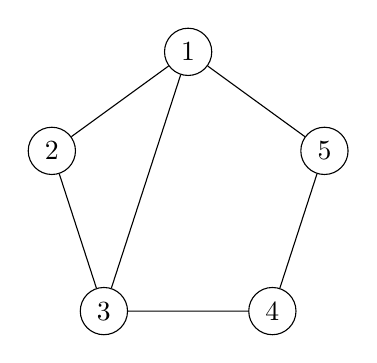
\begin{tikzpicture}[scale=1.3, every node/.style={circle, draw, minimum size=6mm, inner sep=0}]
  \node (v1) at (90:1.4)   {1};
  \node (v2) at (162:1.4)  {2};
  \node (v3) at (234:1.4)  {3};
  \node (v4) at (306:1.4)  {4};
  \node (v5) at (18:1.4)   {5};
  \draw (v1) -- (v2) -- (v3) -- (v4) -- (v5) -- (v1);
  \draw (v1) -- (v3);
\end{tikzpicture}
\end{center}

\section{Combinatorics basics}

\begin{definition}
The number of ways to choose an (unordered) subset of $k$ elements from a
set of $n$ elements is the \emph{binomial coefficient}
\[
  \binom{n}{k} = \frac{n!}{k!\,(n-k)!}.
\]
\end{definition}

\begin{theorem}[Pascal's rule]
\[
  \binom{n}{k} = \binom{n-1}{k-1} + \binom{n-1}{k}
\]
\end{theorem}

\begin{proof}
Fix one element $x$ of the $n$-set. A $k$-subset either contains $x$ — in
which case the rest is a $(k-1)$-subset of the remaining $n-1$ elements —
or it doesn't, in which case it's a $k$-subset of those $n-1$ elements.
These cases are disjoint and exhaustive, so the counts add.
\end{proof}

\begin{theorem}[Pigeonhole principle]
If $n$ items are placed into $m$ containers and $n > m$, at least one
container holds more than one item.
\end{theorem}

\begin{proof}
Suppose not: every container holds at most one item. Then the total number
of items is at most $m$. But $n > m$, a contradiction.
\end{proof}

The pigeonhole principle looks almost too simple to be useful, but it
reappears constantly in graph theory: in a simple graph on $n \geq 2$
vertices, two vertices must share the same degree, because there are only
$n - 1$ possible degree values $(0, \dots, n-1)$ available to distribute
among the $n$ vertices, and $0$ and $n-1$ can never both occur together —
so effectively $n - 1$ ``containers'' for $n$ ``items''.

\section{Try it}

Extend Section 3: add a sixth vertex connected to two existing ones, and
recompute $V$, $E$, and $F$ by hand before checking Euler's formula still
holds. Recompile (right-click, compile LaTeX again) to see the updated
figure.

\end{document}
